\documentclass[aspectratio=169,11pt]{beamer}

% Shared style (ib-tutorials.sty at the repo root).
\makeatletter\def\input@path{{./}{../}}\makeatother
\usepackage{ib-tutorials}

\usepackage[utf8]{inputenc}
\usepackage{amsmath,amssymb}
\usepackage{booktabs}
\usepackage{array}
\newcolumntype{L}[1]{>{\raggedright\arraybackslash}p{#1}}
\usepackage{graphicx}
\graphicspath{{../pictures/4-ibfe/}{pictures/4-ibfe/}}
\usepackage{xcolor}
\usepackage{listings}
\usepackage{tikz}
\usetikzlibrary{arrows.meta,positioning,shapes.geometric,fit,calc,decorations.pathmorphing}
\usepackage{hyperref}

\newcommand{\sourcecredit}[1]{\vfill\begin{flushright}\tiny\textcolor{DarkGray}{#1}\end{flushright}}

\lstset{
  basicstyle=\ttfamily\scriptsize\color{BlackGray},
  keywordstyle=\color{NavyBlue}\bfseries,
  commentstyle=\color{DarkGray}\itshape,
  stringstyle=\color{OliveGreen},
  showstringspaces=false,
  columns=fullflexible,
  keepspaces=true,
  breaklines=true,
  breakindent=1em,
  frame=single,
  framerule=0.4pt,
  rulecolor=\color{LightGray},
  backgroundcolor=\color{LightGray!30},
  xleftmargin=0.25em,
  xrightmargin=0.25em
}
\lstdefinestyle{shell}{morecomment=[l]{\#}}
\lstdefinestyle{input}{morecomment=[l]{//}}
\lstdefinestyle{matlab}{morecomment=[l]{\%}}
\lstdefinestyle{python}{morecomment=[l]{\#}}
\lstdefinestyle{data}{}
\lstdefinestyle{tiny}{basicstyle=\ttfamily\tiny\color{BlackGray}}
\lstdefinestyle{inputtiny}{morecomment=[l]{//},basicstyle=\ttfamily\tiny\color{BlackGray}}
\lstdefinestyle{cpp}{language=C++,morecomment=[l]{//}}
\lstdefinestyle{cpptiny}{language=C++,morecomment=[l]{//},basicstyle=\ttfamily\tiny\color{BlackGray}}

\title[Two or more meshes]{Two or more meshes}
\subtitle{Parts in \code{IBFEMethod}: one mesh file per body or one file placed twice, per-part registration and output, a plate driven into a free disc (IBFE/08), the 2020 clap-and-fling wings with their kinematics corrected, and the two-body technique of the 2018 coral example}
\author[Miller]{Laura A. Miller}
\institute[UArizona]{Department of Mathematics, University of Arizona}
\date{Using IB Software \textbullet\ Part IV \textbullet\ Chapter 21}

\begin{document}

% 1
\begin{frame}[plain]
\maketutorialtitlepanel{%
\begin{tikzpicture}[scale=0.84]
  % a disc above an upright plate
  \draw[BlackGray,thick] (1.3,2.0) circle (0.42);
  \foreach \a in {0,30,...,150} \draw[BlackGray,thin] (1.3,2.0) ++(\a:0.42) -- ++(\a+180:0.84);
  \draw[BlackGray,thick] (1.22,0.3) rectangle (1.38,1.2);
  \foreach \y in {0.4,0.55,...,1.1} \draw[BlackGray,thin] (1.22,\y) -- (1.38,\y);
  \draw[-{Stealth[length=2mm]},RubineRed,very thick] (1.3,0.05) -- (1.3,-0.3+0.6);
  \node[font=\tiny,text=RubineRed] at (0.6,0.5) {part 0: tether};
  \node[font=\tiny,text=NavyBlue] at (2.4,2.1) {part 1: free};
  \node[font=\tiny,text=DarkGray] at (3.0,1.1) {\code{meshes = \{\&beam, \&circle\}}};
  \node[font=\tiny,text=DarkGray] at (3.0,0.75) {\code{register*(data, part)}};
  \node[font=\tiny,text=OliveGreen] at (3.0,0.4) {\code{beam\_output.ex2}, \code{circle\_output.ex2}};
\end{tikzpicture}}
\end{frame}

% 2
\begin{frame}{Learning goals}
\label{fr:goals}
\footnotesize By the end of this chapter you should be able to:
\begin{enumerate}
  \item give \code{IBFEMethod} several meshes (``parts''), register stress and force functions part by part, and write one ExodusII file per part, with the prefix mechanism that names them;
  \item choose between two mesh files, one file read twice and placed by coordinate mappings, and one mesh with subdomains, and say when each is right;
  \item build and run IBFE/08, a tethered plate driven into a free disc, and read from its two output files how close the two bodies get and why the disc keeps moving;
  \item read the 2020 clap-and-fling wing example: two wings, two target functions, the same stress, $\kappa_s = 10^{13}$, and the half-stroke switch in its kinematics that leaves the target's velocity discontinuous; write the corrected rigid-wing kinematics the 2020 slide promised;
  \item describe the 2018 two-coral technique (CAD to a hex mesh, one body placed twice, a bell-like bending motion) and reproduce it with a neutral body;
  \item look at several parts at once in VisIt, and restart a multi-part run without damaging its files.
\end{enumerate}
\begin{punchbox}
\footnotesize Everything of chapters 17--20 was one mesh. Here the only new word is \emph{part}: an index that every registration, every data manager and every output file carries.
\end{punchbox}
\end{frame}

% 3
\begin{frame}{Where this chapter comes from}
\label{fr:sources}
\scriptsize
\begin{itemize}
  \item \al{``6-IBFE: Two Meshes'' (2015, edited 2018; 6 slides):} ``Random info'', the ca.-2016 two-mesh code (\code{getExodusIIFilename("mesh1")}, \code{vector<Mesh*> meshes}, per-part registration, two \code{AutoPtr<ExodusII\_IO>}), and ``Laura's Notes'' on the constructor and \code{postprocess\_data}. The 2020 ``Plans for June'' deck repeats the code as the ``ca.\ 2016 approach''.
  \item \al{``7-IBFE: Two Boundaries: Flapping wings and beam hits circle'' (2020; 20 slides):} the 3D clap-and-fling wings (Trelis meshes, prescribed sweep and angle of attack, a target function per wing) and the 2D beam driven into a circle, with the current \code{std::vector<MeshBase*>} and \code{std::unique\_ptr} code. Example IBFE/08 is the second; the first is \code{examples/legacy/UNC-Examples/7-IBFE-TwoWings}.
  \item \al{The 2016 example \code{Example\_IBFE\_TetherForceMultiplePlate2D} (course set 2016-11):} the ``\ldots multipleplate2d'' of the 2015 slide: one plate mesh read twice, placed by two coordinate mappings, each copy with its own target function.
  \item \al{``2-IBFE Detailed Example using Target Points in 3D'' (MATH 769, 2018; 14 slides, private):} two pulsing corals, Fusion 360 $\to$ Bolt hex mesh $\to$ two copies placed by coordinate mappings $\to$ a bell-like bending motion with a contraction and an expansion phase. The deck ends before the code it promises; the coral research model is not in the public collection. Its technique is taught here with a neutral body (slide \ref{fr:corals}).
  \item \al{New here:} the \code{IBFEMethod} constructor and \code{AppInitializer::getExodusIIFilename(prefix)} from the source; the registration table for several parts; IBFE/08's measured results and figures; the wing kinematics analysed (continuous position, discontinuous velocity at each half-stroke; the thickness sheared) and corrected; restart with several parts; VisIt with several databases; upstream ex6 and ex8 as further patterns.
\end{itemize}
\end{frame}

% 4
\begin{frame}[fragile]{A part is an index}
\label{fr:part}
\scriptsize
\begin{lstlisting}[style=cpptiny]
IBFEMethod(const std::string& object_name, const SAMRAI::tbox::Pointer<SAMRAI::tbox::Database>& input_db,
           libMesh::MeshBase* mesh, int max_levels, bool register_for_restart = true,
           const std::string& restart_read_dirname = "", unsigned int restart_restore_number = 0);      // one mesh
IBFEMethod(const std::string& object_name, const SAMRAI::tbox::Pointer<SAMRAI::tbox::Database>& input_db,
           const std::vector<libMesh::MeshBase*>& meshes, int max_levels, bool register_for_restart = true,
           const std::string& restart_read_dirname = "", unsigned int restart_restore_number = 0);      // several
\end{lstlisting}
\begin{tabular}{@{}L{0.34\textwidth}L{0.58\textwidth}@{}}
\toprule
where the part appears & what it means \\
\midrule
the order of \code{meshes} & part $0$ is \code{meshes[0]}, part $1$ is \code{meshes[1]}, \ldots; the one-mesh constructor is the vector of length one \\
\code{register*(data, part)} & every registration function of chapter 19 takes the part as its last argument (default $0$): stress functions, body, surface and pressure forces, coordinate mapping, initial velocity \\
\code{getFEDataManager(part)} & each part has its own \code{FEDataManager}, equation systems, and quadrature settings; \code{->getEquationSystems()} is what its ExodusII writer writes \\
one \code{ExodusII\_IO} per part & each writer is built on its own mesh and writes its own file (slide \ref{fr:exodus}) \\
\code{elem->subdomain\_id()} & is \emph{not} a part: subdomains live inside one mesh (chapter 18) and are told apart inside a stress function \\
\bottomrule
\end{tabular}

\medskip
The input file does not know about parts: one \code{IBFEMethod} block serves all of them (\code{IB\_point\_density}, the kernel, \code{split\_forces} apply to every part).
\end{frame}

% 5
\begin{frame}{Three ways to get two bodies}
\label{fr:ways}
\scriptsize
\begin{tabular}{@{}L{0.24\textwidth}L{0.36\textwidth}L{0.32\textwidth}@{}}
\toprule
way & how & used by \\
\midrule
A. two mesh files & \code{beam\_mesh.read("beam.e")}, \code{circle\_mesh.read("circle.e")}, two entries in \code{meshes} & IBFE/08; the two wings (\code{pos\_wing.e}, \code{neg\_wing.e}); upstream ex6 and ex8 build theirs in the program \\
B. one file, read twice, placed twice & two \code{Mesh} objects read the same file; a coordinate mapping per part puts each copy where it belongs (\code{X = s + shift}, or a rotation) & the 2016 two-plate example (slide \ref{fr:multi}); the 2018 corals (slide \ref{fr:corals}) \\
C. one mesh, two subdomains & one part; the mesher's physical groups or Exodus blocks give the elements ids; the stress function tests \code{elem->subdomain\_id()} & a stem and a leaf, a wall and its stiff band; chapter 18, slide 26 \\
\bottomrule
\end{tabular}

\medskip
\begin{itemize}
  \item A and B are parts: each body can have its own forces, its own output file, its own stress; the bodies do not share nodes and can touch, separate or pass each other. The fluid between them is what keeps them apart (IBFE/08's plate never touches the disc, slide \ref{fr:results}).
  \item C is one body with two materials: the two regions are joined, strain passes from one to the other, and there is one output file. Use it for a body with a stiff and a soft region, not for two bodies.
  \item B saves a mesh file and guarantees identical bodies; A lets the bodies differ. Both need a coordinate mapping only if the file is not already where the body should start (chapter 22 has the mapping in full).
\end{itemize}
\end{frame}

% 6
\begin{frame}[fragile]{IBFE/08: a plate driven into a free disc}
\label{fr:example}
\scriptsize
\begin{columns}[T]
\column{0.5\textwidth}
``In this example, a 2D beam is propelled towards a 2D circle. Target points drive the beam for the first 1 second, and then the beam is free to coast. The circle is untethered and moves due to the approaching beam'' (2020, slide 15).
\begin{itemize}
  \item Domain $2\times2$, periodic; two levels, $32 \to 128$ cells; fluid $\rho = 1$, $\mu = 0.01$.
  \item Part 0, the plate: $0.0312$ wide, $0.5$ tall, upright, centre $(0, -0.5)$: \code{beam.e}, $98$ nodes, $126$ \code{TRI3}, made with Trelis.
  \item Part 1, the disc: radius $0.25$, centre $(0, 0.5)$: \code{circle.e}, $977$ nodes, $1851$ \code{TRI3}. Its bottom starts $0.5$ above the plate's top.
  \item Both neo-Hookean, $\mu = 10$ (\code{SHEAR\_MODULUS}); the plate's tether moves up at \code{TETHER\_SPEED = 0.25} until \code{TETHER\_END\_TIME = 1.0}, $\kappa_s = 10^6$; the disc has no tether.
  \item $8000$ steps of \code{DT = 5e-4}; $81$ frames, one every $0.05$ (\code{viz\_dump\_interval = int(.05/DT)}, the 2015 slide's tip); about two minutes on four cores.
\end{itemize}
\column{0.48\textwidth}
\begin{lstlisting}[style=cpptiny]
// the tether on the plate (part 0) only
void beam_tether_force_function(VectorValue<double>& F, ..., const libMesh::Point& X,
                                const libMesh::Point& s, ..., double time, void* /*ctx*/)
{
    libMesh::Point s_target = X;                  // no force by default
    if (time < tether_end_time)
    {
        s_target(0) = s(0);
        s_target(1) = s(1) + tether_speed * time; // up at 0.25
    }
    F = kappa_s * (s_target - X);
}
\end{lstlisting}
\scriptsize The 2020 slide 17 is the same with \code{.25*time} and \code{time < 1} written in.
\end{columns}
\end{frame}

% 7
\begin{frame}[fragile]{IBFE/08 (2): the two meshes and the parts}
\label{fr:code}
\begin{lstlisting}[style=cpptiny]
// Each part gets its own ExodusII file: viz_IB2d/beam_output.ex2 and viz_IB2d/circle_output.ex2.
const bool uses_exodus = dump_viz_data && !app_initializer->getExodusIIFilename().empty();
const string beam_exodus_filename = app_initializer->getExodusIIFilename("beam_");
const string circle_exodus_filename = app_initializer->getExodusIIFilename("circle_");
...
// Read the two meshes. libMesh chooses the reader from the file name; .e is an ExodusII file.
// The order of the meshes in the vector sets the part numbers: the plate is part 0 and the disc is part 1.
Mesh beam_mesh(init.comm(), NDIM);
beam_mesh.read(input_db->getStringWithDefault("BEAM_MESH_FILENAME", "beam.e"));
beam_mesh.prepare_for_use();
Mesh circle_mesh(init.comm(), NDIM);
circle_mesh.read(input_db->getStringWithDefault("CIRCLE_MESH_FILENAME", "circle.e"));
circle_mesh.prepare_for_use();
std::vector<MeshBase*> meshes = { &beam_mesh, &circle_mesh };
...
Pointer<IBFEMethod> ib_method_ops = new IBFEMethod("IBFEMethod", app_initializer->getComponentDatabase("IBFEMethod"),
                                                   meshes, max_levels, /*register_for_restart*/ true,
                                                   restart_read_dirname, restart_restore_num);
...
// Configure the IBFE solver. The last argument of each register call is the part number.
// Both parts get the same stress functions; only the plate (part 0) gets the tether force.
ib_method_ops->registerLagBodyForceFunction(beam_tether_force_data, 0);
ib_method_ops->registerPK1StressFunction(PK1_dev_stress_data, 0);
ib_method_ops->registerPK1StressFunction(PK1_dil_stress_data, 0);
ib_method_ops->registerPK1StressFunction(PK1_dev_stress_data, 1);
ib_method_ops->registerPK1StressFunction(PK1_dil_stress_data, 1);
ib_method_ops->initializeFEEquationSystems();
EquationSystems* beam_equation_systems = ib_method_ops->getFEDataManager(0)->getEquationSystems();
EquationSystems* circle_equation_systems = ib_method_ops->getFEDataManager(1)->getEquationSystems();
\end{lstlisting}
\end{frame}

% 8
\begin{frame}[fragile]{IBFE/08 (3): one ExodusII writer per part, and the restart rule}
\label{fr:exodus}
\footnotesize
\begin{lstlisting}[style=cpptiny]
// Set up visualization plot file writers: one ExodusII writer per part.
std::unique_ptr<ExodusII_IO> beam_exodus_io = uses_exodus ? std::make_unique<ExodusII_IO>(beam_mesh) : nullptr;
std::unique_ptr<ExodusII_IO> circle_exodus_io = uses_exodus ? std::make_unique<ExodusII_IO>(circle_mesh) : nullptr;
// A restarted run adds its time steps to the existing ExodusII files. Only processor 0 writes the files, so only
// processor 0 reopens them: libMesh 1.7.8 reopens them on every processor when told to append, and with more than
// one process the files are then damaged (they can no longer be read).
if (uses_exodus)
{
    const bool from_restart = RestartManager::getManager()->isFromRestart();
    beam_exodus_io->append(from_restart && IBTK_MPI::getRank() == 0);
    circle_exodus_io->append(from_restart && IBTK_MPI::getRank() == 0);
}
...   // in the time loop, at every dump:
beam_exodus_io->write_timestep(beam_exodus_filename, *beam_equation_systems, iteration_num / viz_dump_interval + 1, loop_time);
circle_exodus_io->write_timestep(circle_exodus_filename, *circle_equation_systems, iteration_num / viz_dump_interval + 1, loop_time);
\end{lstlisting}
\begin{itemize}
  \item \code{getExodusIIFilename(prefix)} returns \code{viz\_dump\_dirname + "/" + prefix + exodus\_filename} (\code{AppInitializer.cpp}): the prefix is glued to the file name (\code{output.ex2} unless the \code{Main} database sets \code{exodus\_filename}) with no separator. The course wrote \code{"mesh1"} and got \code{mesh1output.ex2}; the example writes \code{"beam\_"} and gets \code{beam\_output.ex2}. Two parts with no prefix would write the same file twice.
\end{itemize}
\end{frame}

% 8b
\begin{frame}{IBFE/08 (3b): dumps and restarts with two parts}
\label{fr:restart}
\footnotesize
\begin{itemize}
  \item One \code{write\_timestep} per part at every dump, with the same time-state number; both files hold $81$ states here ($0.6$ MB for the plate, $5.2$ MB for the disc). A part written at a different interval would need VisIt's database correlation to line up (slide \ref{fr:visit}).
  \item \code{register\_for\_restart = true} in the constructor saves and reloads the finite element data of every part with the fluid's restart files; a restarted run then appends its new states to both ExodusII files. The shipped input has \code{restart\_dump\_interval = 0}; \code{int(0.5/DT)} writes a restart every half time unit.
  \item The restart rule is IBFE/08's own finding (0.16.0 and 0.19.0): IBAMR's examples pass \code{append(from\_restart)} on every rank, and a restart on more than one process leaves files that VisIt cannot open. Only rank $0$ writes, so only rank $0$ reopens.
  \item The same rule holds with one part; it only shows up more often with several, because multi-part runs are the long ones that get restarted.
\end{itemize}
\end{frame}

% 9
\begin{frame}{IBFE/08 (4): what happens}
\label{fr:pics}
\begin{columns}[T]
\column{0.25\textwidth}\centering 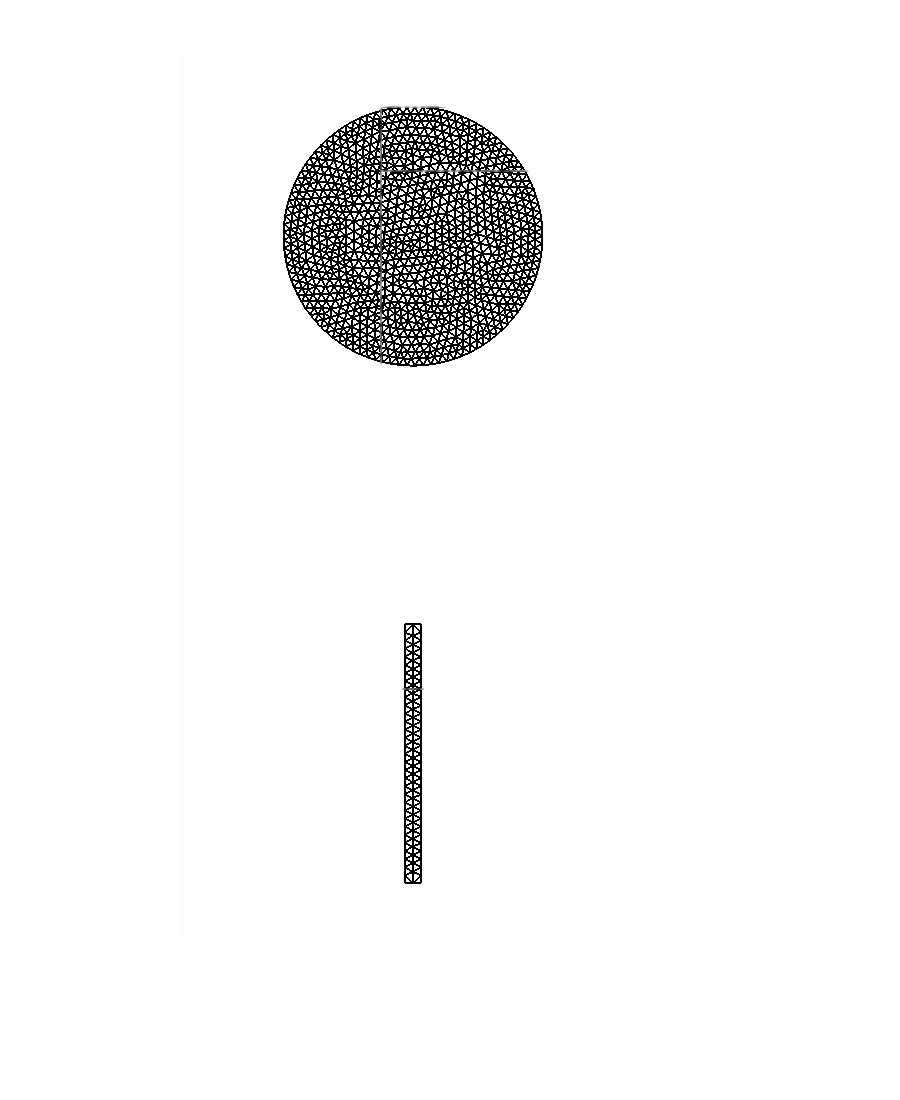
\includegraphics[width=0.78\textwidth]{ch21-hit-t0.png}\\ \scriptsize $t = 0$: gap $0.500$
\column{0.25\textwidth}\centering 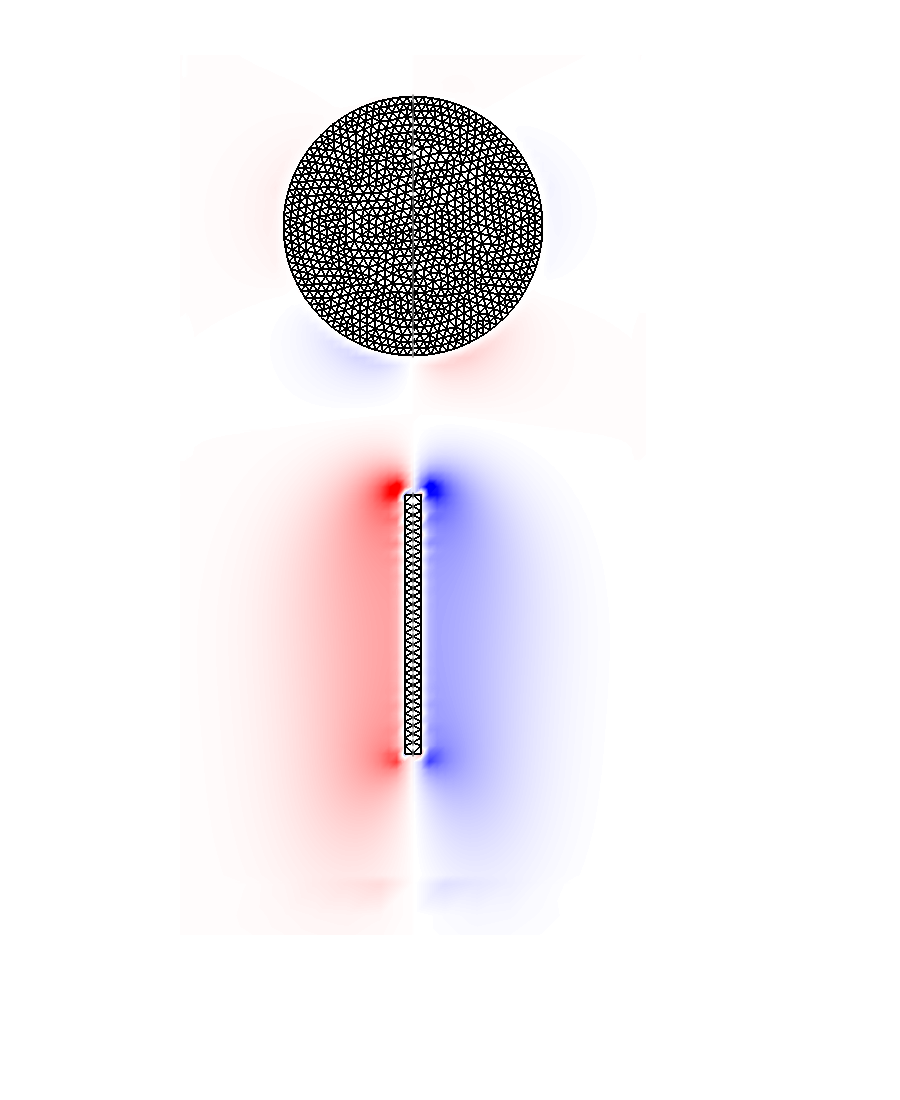
\includegraphics[width=0.78\textwidth]{ch21-hit-t1.png}\\ \scriptsize $t = 1$: released; gap $0.269$
\column{0.25\textwidth}\centering 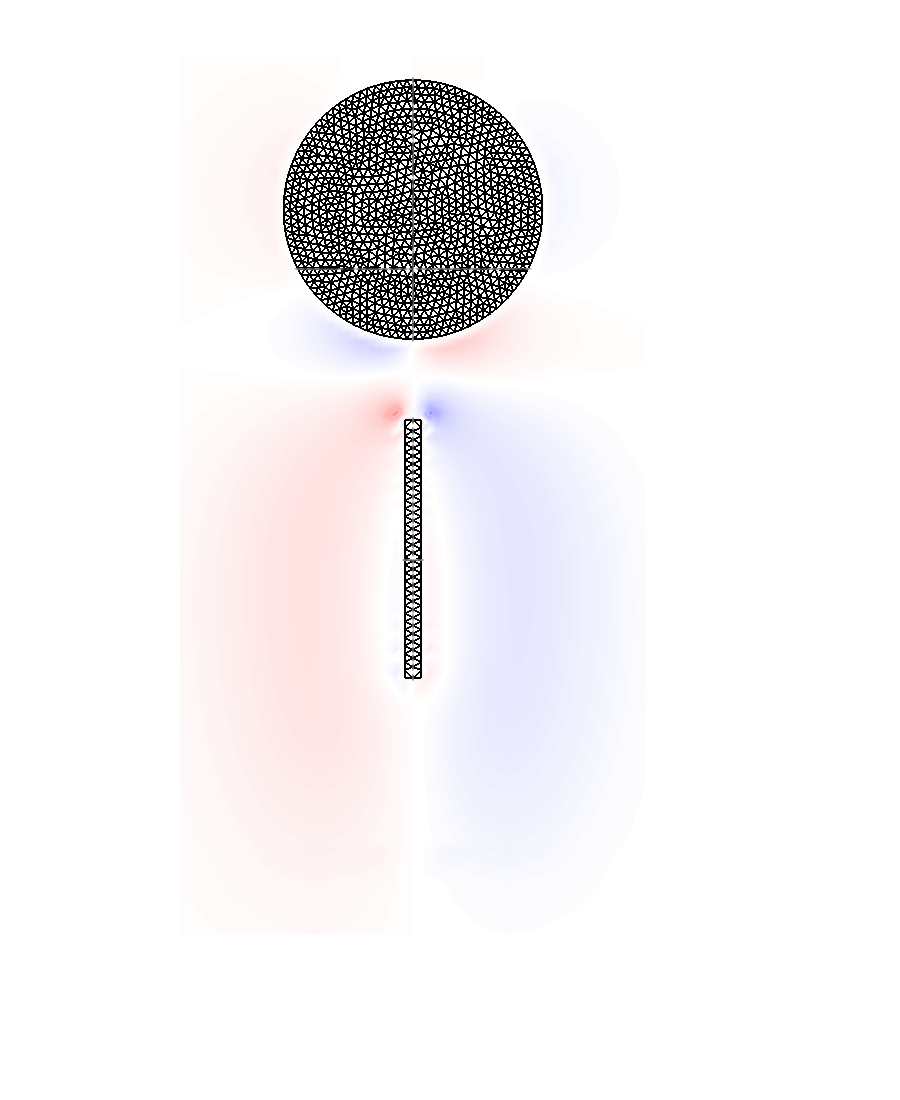
\includegraphics[width=0.78\textwidth]{ch21-hit-t2.png}\\ \scriptsize $t = 2$: gap $0.156$
\column{0.25\textwidth}\centering 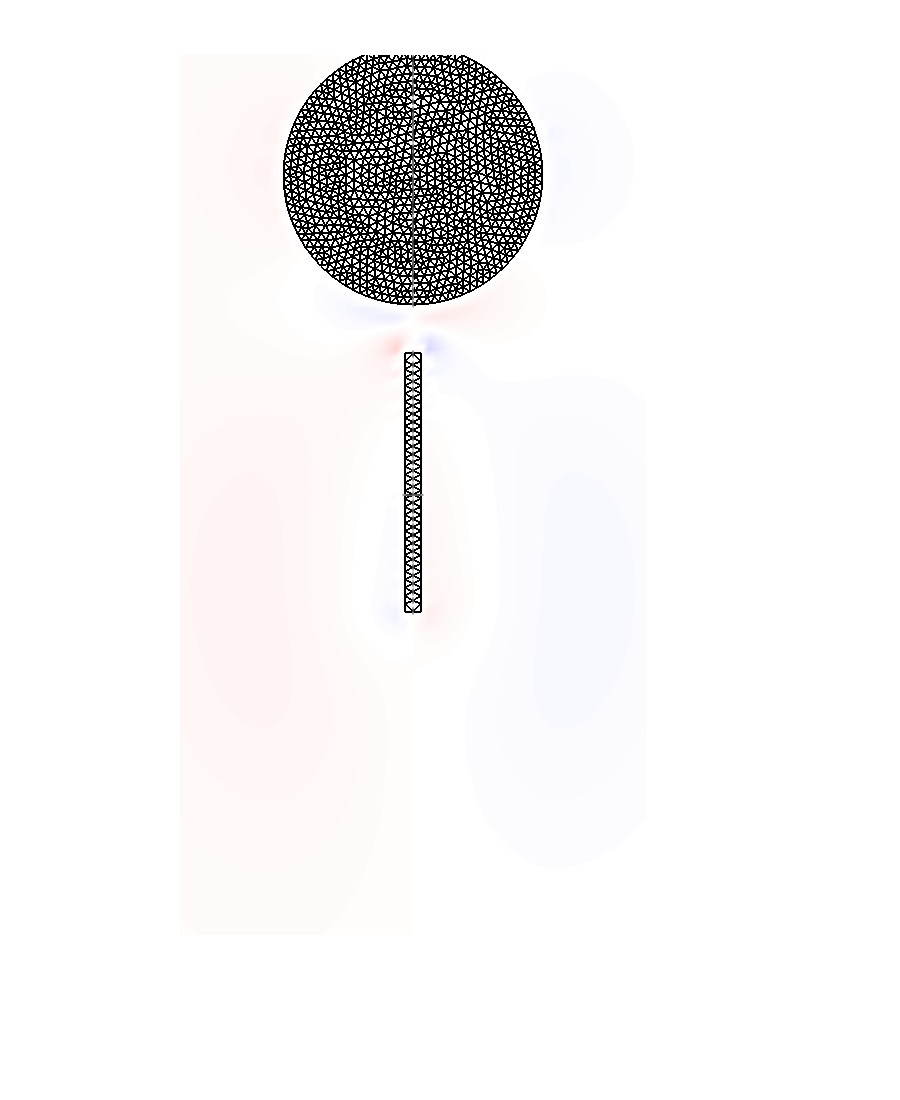
\includegraphics[width=0.78\textwidth]{ch21-hit-t4.png}\\ \scriptsize $t = 4$: gap $0.094$
\end{columns}
\scriptsize
\begin{itemize}
  \item Vorticity $\pm5$ on the fluid grid; the two meshes, each displaced by its own \code{dX}. Window $[-0.45, 0.45]\times[-0.85, 0.85]$.
  \item The plate is pushed up for one second and coasts; the disc moves because the fluid the plate pushed moves it. The vorticity pair at the plate's top is the wake of a blunt body; the disc deforms hardly at all (its width stays $0.500$).
\end{itemize}
\sourcecredit{IBFE/08, IBAMR 0.19.0 (\code{/root/work/0.19.0/ibfe08\_final}); \code{wsl/final/visit\_ch21.sh}.}
\end{frame}

% 10
\begin{frame}{IBFE/08 (5): the numbers, and why the disc keeps moving}
\label{fr:results}
\footnotesize
From the two ExodusII files (plate top: its highest nodes; disc bottom: its lowest):
\begin{tabular}{@{}lllll@{}}
\toprule
time & plate top $y$ & disc bottom $y$ & gap & \\
\midrule
$0$ & $-0.250$ & $0.250$ & $0.500$ & \\
$1.0$ & $0.000$ & $0.270$ & $0.269$ & the plate is released; its top is where the target put it \\
$2.0$ & $0.146$ & $0.301$ & $0.156$ & \\
$3.0$ & $0.222$ & $0.335$ & $0.113$ & \\
$4.0$ & $0.274$ & $0.368$ & $0.094$ & about six fine grid cells \\
\bottomrule
\end{tabular}

\medskip
\begin{itemize}
  \item While tethered the plate follows its target to three digits. Released, it keeps rising more and more slowly, and the gap keeps closing, but the plate does not reach the disc: the disc is moving away too.
  \item Why: the tether pushes the plate, and through it the fluid, upward. In a periodic box that momentum has nowhere to go; after $t = 1$ the average upward velocity of the whole fluid stays at $0.016$ ($0.0162$ at $t = 1$, $0.0159$ at $t = 4$, from the VisIt files). The disc sits in the column of fluid above the plate and rises at about $0.033$. A periodic box is not a tank: chapter 7's boundary conditions, or a longer box, change this.
  \item \code{TETHER\_END\_TIME = 2.0} (the README's ``Things to try''): the plate's top reaches $y = 0.250$ at $t = 2$ and the gap closes to $0.040$ at $t = 2.5$, about $2.6$ fine cells, then stays near $0.045$: the fluid between them keeps them apart, and the disc is squeezed a little (width $0.5006$). Next slide.
  \item 0.16.0 and 0.19.0 agree to $2\times10^{-8}$ in the node positions.
\end{itemize}
\end{frame}

% 11
\begin{frame}{IBFE/08 (6): pushing longer}
\label{fr:push2}
\begin{columns}[T]
\column{0.3\textwidth}\centering 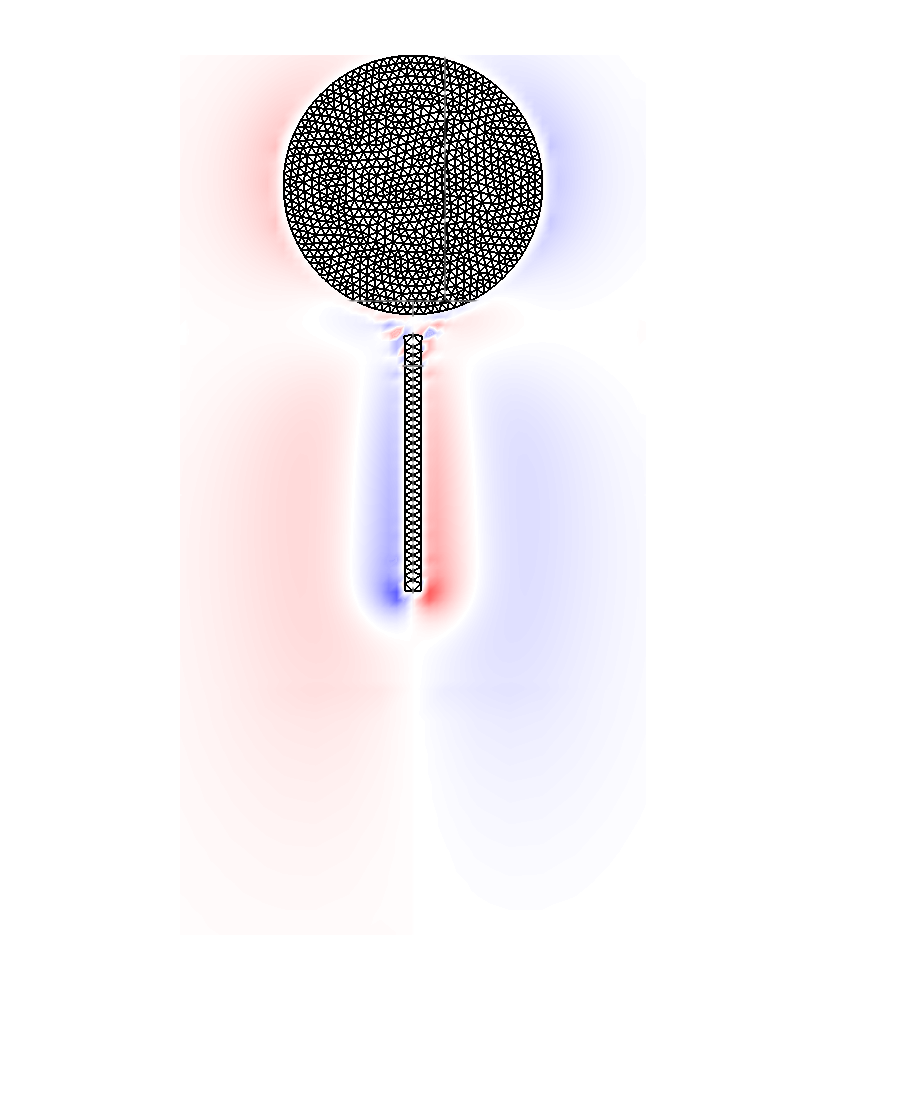
\includegraphics[width=0.8\textwidth]{ch21-push2-t25.png}\\ \scriptsize \code{TETHER\_END\_TIME = 2}, $t = 2.5$: gap $0.040$
\column{0.3\textwidth}\centering 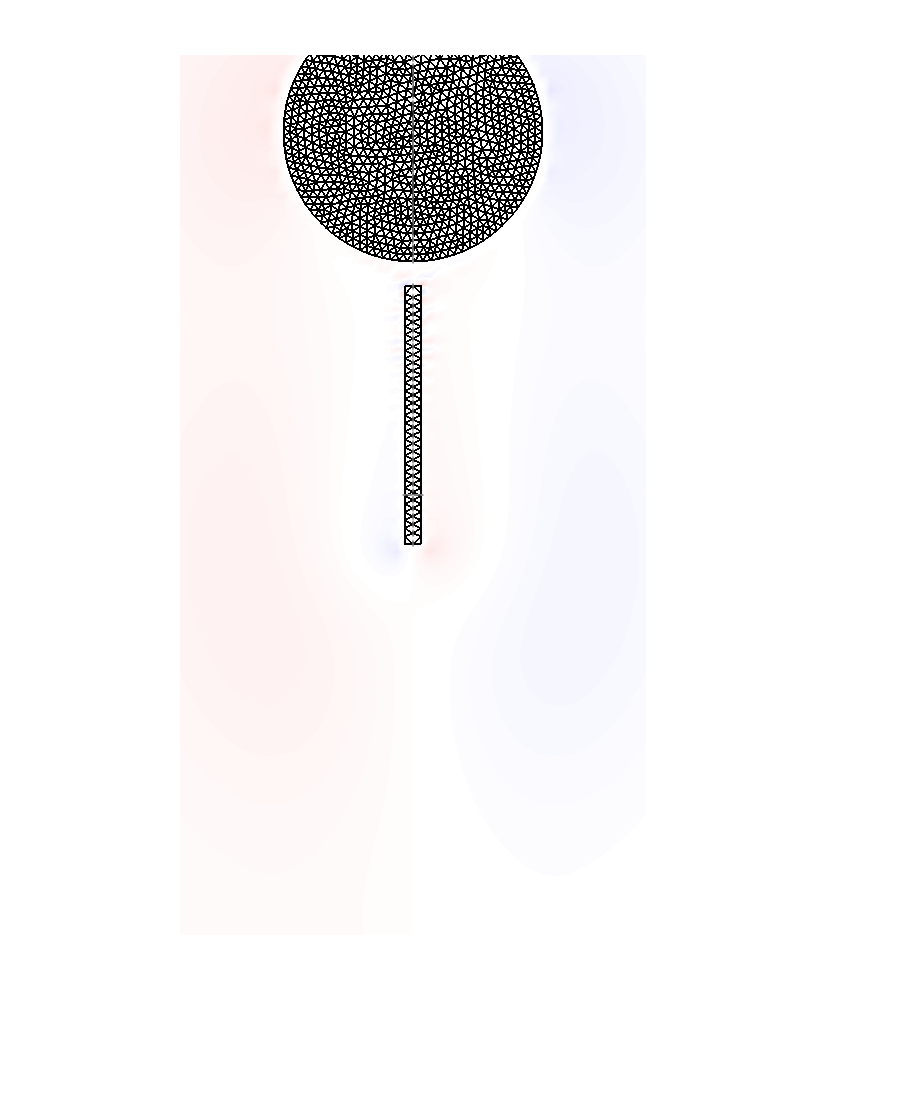
\includegraphics[width=0.8\textwidth]{ch21-push2-t4.png}\\ \scriptsize $t = 4$: gap $0.045$
\column{0.4\textwidth}
\scriptsize
\begin{itemize}
  \item The two bodies come within three fine grid cells and stay there. There is no contact model in IBFE: the fluid film between them, resolved by two or three cells, carries the load. Closer than that, the two bodies' quadrature points spread force into the same cells and the film can no longer thin; the point method of Part II behaves the same way.
  \item Real contact (a valve leaflet on its seat, two corals brushing) needs a thinner film resolved by a finer grid, or a penalty between the surfaces written as surface forces (chapter 19, slide 24) that test the other body's position through \code{ctx}.
  \item The disc's width grows to $0.5006$ at $t = 2$: it is being pressed; its own neo-Hookean stress pushes back.
\end{itemize}
\end{columns}
\sourcecredit{\code{/root/work/0.19.0/ibfe08\_push2}, IBAMR 0.19.0.}
\end{frame}

% 12
\begin{frame}[fragile]{The 2016 two-plate example: one file, read twice, placed by coordinate mappings}
\label{fr:multi}
\footnotesize
\code{Example\_IBFE\_TetherForceMultiplePlate2D} (course set 2016-11; the ``\ldots multipleplate2d'' of the 2015 slide):
\begin{lstlisting}[style=cpptiny]
void coordinate1_mapping_function(libMesh::Point& X, const libMesh::Point& s, void* /*ctx*/)
{   X(0) = s(1)+.2;  X(1) = s(0);  return; }          // the plate turned upright and put at x = +0.2
void coordinate2_mapping_function(libMesh::Point& X, const libMesh::Point& s, void* /*ctx*/)
{   X(0) = s(1)-.2;  X(1) = s(0);  return; }          // its twin at x = -0.2
void target1_force_function(..., const libMesh::Point& X, const libMesh::Point& s, ..., double time, ...)
{   libMesh::Point s_dump;
    if(time<1)      { s_dump(0)=s(1)+.2+.5*time;        s_dump(1)=s(0); }   // move right at 0.5
    else if(time<2) { s_dump(0)=s(1)+.2+.5+.5*(1-time); s_dump(1)=s(0); }   // and back
    else            { s_dump(1)=X(1); s_dump(0)=X(0); }
    F = kappa_s*(s_dump-X); return; }
// target2_force_function: the mirror image, s(1)-.2-.5*time, ...
...
mesh1.read("IBFE_Mesh2D_128.mat");  mesh1.prepare_for_use();
mesh2.read("IBFE_Mesh2D_128.mat");  mesh2.prepare_for_use();
vector<Mesh*> meshes(2);  meshes[0] = &mesh1;  meshes[1] = &mesh2;
...
ib_method_ops->registerInitialCoordinateMappingFunction(coordinate1_mapping_function, 0);
ib_method_ops->registerInitialCoordinateMappingFunction(coordinate2_mapping_function, 1);
ib_method_ops->registerLagBodyForceFunction(target1_force_data, 0);
ib_method_ops->registerLagBodyForceFunction(target2_force_data, 1);
\end{lstlisting}
\end{frame}

% 12b
\begin{frame}{The 2016 two-plate example (2): what the mappings and the targets do}
\label{fr:multi2}
\footnotesize
\begin{itemize}
  \item The mapping swaps the axes, so the horizontal plate of chapter 17 stands upright, and shifts each copy sideways; the two plates then move apart at $0.5$ for a second and back for a second: a pair of paddles. The target functions must apply the same mapping to \code{s} (``\code{s(1)+.2}''), because \code{s} is the \emph{file's} reference position, not the mapped one: chapter 22 makes this precise.
  \item Each copy has its own target function, registered on its own part; the two functions differ only in the sign of the shift and of the motion. One function with the part's shift passed through \code{ctx} (chapter 19, slide 23) would do the same with less code.
  \item At $t = 0$ the plates stand $0.4$ apart; at $t = 1$, $1.4$ apart; at $t = 2$ they are back. After $t = 2$ the target is the current position, so the tether does nothing and the plates are free (exercise 4).
  \item This is the pattern the two-coral deck followed two years later with a 3D hex mesh (slide \ref{fr:corals}).
\end{itemize}
\end{frame}

% 13
\begin{frame}[fragile]{The 2015 and 2020 notes, and the code they corrected}
\label{fr:notes}
\scriptsize
\begin{columns}[T]
\column{0.5\textwidth}
``Random info'' (2015):
\begin{itemize}
  \item ``Example \ldots multipleplate2d''; ``VisIt $\to$ make first after adding dumps.visit stuff'' (the Draw button, so that the fluid's time axis exists before the Exodus databases are added);
  \item ``copies of everything with coordinate mappings in main.C'';
  \item ``\code{viz\_dump\_interval = int(0.05/DT)} helpful in input2d/input3d in general'' (IBFE/08 uses it: a dump every $0.05$ whatever \code{DT} is).
\end{itemize}
``Laura's Notes'' (2015): ``Mesh needs to be changed to meshes on this line'', the constructor with \code{meshes}; ``also need to change meshes here as well as equation systems'' in \code{postprocess\_data}, which took one mesh and one \code{EquationSystems}: with two parts it wrote one of them.
\column{0.48\textwidth}
The 2020 deck's ``Other changes from earlier versions'':
\begin{lstlisting}[style=cpptiny]
// these lines
AutoPtr<ExodusII_IO> mesh1_exodus_io(uses_exodus ? new ExodusII_IO(mesh1) : NULL);
// should be changed to these lines
std::unique_ptr<ExodusII_IO> mesh1_exodus_io(uses_exodus ? new ExodusII_IO(mesh1) : NULL);
\end{lstlisting}
and, in \code{postprocess\_data}, ``you may need to update the FEBase and QBase lines'':
\begin{lstlisting}[style=cpptiny]
unique_ptr<FEBase> fe(FEBase::build(dim, F_dof_map.variable_type(0)));
unique_ptr<QBase> qrule = QBase::build(QGAUSS, dim, FIFTH);
\end{lstlisting}
\begin{itemize}
  \item \code{vector<Mesh*>} (2015) became \code{std::vector<MeshBase*>} (2020): the constructor takes the base class.
  \item A post-processing function for several parts loops over \code{getFEDataManager(part)} and writes one line per part; chapter 22's flow tank does this for its tether force.
\end{itemize}
\end{columns}
\end{frame}

% 14
\begin{frame}{The 3D clap-and-fling wings (2020): the set-up}
\label{fr:wings}
\footnotesize
\begin{columns}[T]
\column{0.5\textwidth}
\begin{center}
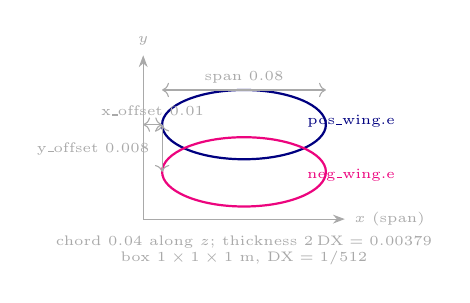
\begin{tikzpicture}[scale=0.8]
  \draw[-{Stealth[length=1.5mm]},DarkGray] (0,0) -- (3.2,0) node[right,font=\tiny] {$x$ (span)};
  \draw[-{Stealth[length=1.5mm]},DarkGray] (0,0) -- (0,2.6) node[above,font=\tiny] {$y$};
  \draw[NavyBlue,thick] (1.6,1.5) ellipse (1.3 and 0.55);
  \draw[RubineRed,thick] (1.6,0.75) ellipse (1.3 and 0.55);
  \node[font=\tiny,text=NavyBlue] at (3.3,1.55) {\code{pos\_wing.e}};
  \node[font=\tiny,text=RubineRed] at (3.3,0.7) {\code{neg\_wing.e}};
  \draw[<->,DarkGray,thin] (0.3,0.75) -- (0.3,1.5); \node[font=\tiny,text=DarkGray,anchor=east] at (0.25,1.12) {\code{y\_offset} $0.008$};
  \draw[<->,DarkGray,thin] (0.3,2.05) -- (2.9,2.05); \node[font=\tiny,text=DarkGray] at (1.6,2.25) {span $0.08$};
  \draw[<->,DarkGray,thin] (0.0,1.5) -- (0.3,1.5); \node[font=\tiny,text=DarkGray] at (0.15,1.72) {\code{x\_offset} $0.01$};
  \node[font=\tiny,text=DarkGray,align=center] at (1.6,-0.5) {chord $0.04$ along $z$; thickness $2\,\mathrm{DX} = 0.00379$\\ box $1\times1\times1$ m, $\mathrm{DX} = 1/512$};
\end{tikzpicture}
\end{center}
\scriptsize Redrawn from the 2020 slide 3 (which wrote $\mathrm{DX} = 1/528 = 0.00189$; the input's $N = 8$, four levels at ratio $4$ give $512$ cells and $0.00195$).
\column{0.48\textwidth}
\begin{itemize}
  \item ``Two elliptical wings performing a simple clap and fling motion. Two separate meshes are uploaded and moved by target forces with different motions. The wings were created using Trelis. This simulation takes a long time to run and generates a lot of data.''
  \item ``I used the trial version of Trelis to make 2 elliptical wings with the right dimensions, rotated and translated them to the correct initial positions. The getting-started tutorial was all I needed to learn enough in under an hour. I exported the meshes as Exodus \code{.e} files.''
\end{itemize}
\end{columns}
\end{frame}

% 14b
\begin{frame}{The wings (2): fluid, material, tether, and the reference axes}
\label{fr:wings2}
\footnotesize
\begin{itemize}
  \item Water (\code{RHO = 1000}), $f = 1$ Hz, and the viscosity set from a target Reynolds number: \code{MU = RHO*(WSPAN/2.0)*((2.0/3.0)*2.0*3.14*WSPAN*FREQUENCY)/RE} with \code{RE = 4}: a tiny insect's regime (chapter 8b).
  \item Compressible neo-Hookean wings with $E = 2$, $\nu = 0.3$ (IBFE/10's law); \code{KAPPA\_S = 1.0e13} (``\code{//5.0e4}'' commented out): the wings are meant to be rigid.
  \item ``Let \code{s(2)} be position along chord and \code{s(0)} be position along span in initial configuration; \code{s(2) = 0} in the middle of the wing'' (2020). Two target functions, one per part, mirror images; the same two stress functions registered on parts $0$ and $1$ (the deck's slide 12: ``applied to mesh 0 / mesh 1 / both meshes'').
  \item \code{DT = 1e-5} with \code{GROW\_DT = 1e-2}: a hundred thousand steps per flapping cycle at $\mathrm{DX} = 1/512$ in 3D, which is why ``this simulation takes a long time to run''; no run of it was made for this chapter.
\end{itemize}
\end{frame}

% 15
\begin{frame}[fragile]{The wings (3): the kinematics, and a target function per wing}
\label{fr:wingcode}
\footnotesize
\begin{lstlisting}[style=cpptiny]
static double kappa_s = 1.0e13; //5.0e4;
static const double freq = 1.0;                  // frequency in hz of flapping
static const double aoa_not = PI/2.0;            // angle of attack at mid-stroke
static const double flap_period = 1.0/freq;
static const double B = PI/4.0;                  // pitch amplitude
static const double sweep_angle = 2.0*PI/3.0;    // sweep amplitude
void target1_force_function(VectorValue<double>& F, ..., const libMesh::Point& X, const libMesh::Point& s, ..., double time, ...)
{
    libMesh::Point s_dump;  double kappa;
    double sweep_angle_pos = 0.5*sweep_angle*(1-cos(2*PI*freq*time));   // sweep: 0 -> 120 deg -> 0 each cycle
    double aoa_pos = aoa_not-B*sin(2*PI*freq*time);                     // pitch: 90 deg -/+ 45 deg
    double chord_length = 0.04;  double offset = 0.01;                  // (offset is never used)
    kappa=kappa_s;  s_dump = s;
    double flap_no = floor(time/flap_period);  double curr_time = time-(flap_no*flap_period);
    if (curr_time<flap_period/2.0){  //downstroke
        s_dump(0) = s(0)*cos(sweep_angle_pos)+((s(2)+0.5*chord_length)*cos(aoa_pos)+s(1))*-sin(sweep_angle_pos);
        s_dump(1) = ((s(2)+0.5*chord_length)*cos(aoa_pos)+s(1))*cos(sweep_angle_pos)+s(0)*sin(sweep_angle_pos);
        s_dump(2) = s(2)*sin(aoa_pos);
    }
    else { //upstroke
        s_dump(0) = s(0)*cos(sweep_angle_pos)+(s(2)*cos(aoa_pos)+s(1))*-sin(sweep_angle_pos);
        s_dump(1) = (s(2)*cos(aoa_pos)+s(1))*cos(sweep_angle_pos)+s(0)*sin(sweep_angle_pos);
        s_dump(2) = s(2)*sin(aoa_pos);
    }
    F = kappa*(s_dump-X);
}
// target2_force_function: the same with sweep_angle_neg = -0.5*sweep_angle*(...) and aoa_neg = aoa_not+B*sin(...)
\end{lstlisting}
\end{frame}

% 16
\begin{frame}{The wings (4): what the kinematics do, and the half-stroke switch}
\label{fr:kinematics}
\footnotesize
The intended motion: the chord vector $(0, 0, s_2)$ is pitched by $\alpha(t)$ into $(0, s_2\cos\alpha, s_2\sin\alpha)$, the thickness $s_1$ is added along $y$, and the result is swept by $\phi(t)$ about the $z$ axis:
\[ \mathbf{X} = \begin{pmatrix} s_0\cos\phi - (s_2\cos\alpha + s_1)\sin\phi \\ (s_2\cos\alpha + s_1)\cos\phi + s_0\sin\phi \\ s_2\sin\alpha \end{pmatrix}, \]
with $\phi = \tfrac12\cdot\tfrac{2\pi}{3}(1 - \cos 2\pi f t)$ and $\alpha = \tfrac{\pi}{2} \mp \tfrac{\pi}{4}\sin 2\pi f t$.
\begin{itemize}
  \item \al{The half-stroke switch.} On the downstroke the code pitches about a point half a chord away (\code{s(2) + 0.5*chord\_length}); on the upstroke about \code{s(2)} itself. At the switch ($t = \tfrac12, 1, \ldots$) $\sin 2\pi ft = 0$, so $\alpha = \tfrac{\pi}{2}$, $\cos\alpha = 0$, and the two formulas give the \emph{same position}: no jump in the target. But their time derivatives differ by $\tfrac{c}{2}\sin\alpha\,\dot\alpha\,(-\sin\phi, \cos\phi, 0)$ with $\dot\alpha = \mp\tfrac{\pi}{2}\cdot 2\pi f$: \al{the target's velocity jumps} by $\tfrac{c}{2}|\dot\alpha| \approx 0.2$ m/s at every half-stroke. With $\kappa_s = 10^{13}$ the plate follows and the fluid sees an impulsive acceleration: a force spike at every half-stroke, and a \code{DT} of $10^{-5}$ to survive it.
\end{itemize}
\end{frame}

% 16b
\begin{frame}{The wings (5): the shear, the pivot, and the unused variables}
\label{fr:shear}
\footnotesize
\begin{itemize}
  \item \al{The shear.} The thickness $s_1$ is added along $y$ \emph{before} the sweep but is not pitched with the chord, so at $\alpha \ne \tfrac{\pi}{2}$ the wing's cross-section is sheared, not rotated: ``these equations work for an infinitely thin wing, but shear a wing that has some thickness. Corrected equations forthcoming'' (2020, slide 6). At $2\,\mathrm{DX}$ thickness the shear is small; the tether at $10^{13}$ enforces it anyway, and the compressible material absorbs it.
  \item \al{The pivot.} Clap-and-fling wings pitch about their leading edge; the leading edge is the same physical edge on both strokes, so one pivot, fixed in the wing, is the kinematics. The switch between two pivots was a way to keep the wing's leading edge in the right place on each stroke; the corrected version below does that by choosing the pivot once and letting $\alpha$ carry the wing through.
  \item \code{offset = 0.01} is computed and unused; \code{flap\_no} and \code{curr\_time} are used only for the switch; \code{kappa = kappa\_s} is a copy that is never changed. These are leftovers of a version that softened the tether near the wing's edge (the \code{//5.0e4}), which is a reasonable thing to do: a tether stiff in the middle and soft at the edge lets the tip flex (chapter 19, slide 26).
\end{itemize}
\end{frame}

% 17
\begin{frame}[fragile]{The wings (6): the corrected rigid-wing kinematics}
\label{fr:corrected}
\scriptsize
A rigid wing is a rotation of its reference shape: pitch the cross-section as a whole, then sweep. With the pivot $p$ along the chord (the leading edge, $p = -c/2$, or the mid-chord, $p = 0$) chosen once:
\[ y_1 = (s_2 - p)\cos\alpha - s_1\sin\alpha,\quad z_1 = (s_2 - p)\sin\alpha + s_1\cos\alpha,\qquad
   \mathbf{X} = \bigl(s_0\cos\phi - y_1\sin\phi,\ \ y_1\cos\phi + s_0\sin\phi,\ \ z_1\bigr). \]
\begin{lstlisting}[style=cpptiny]
static const double pivot = -0.5 * chord_length;   // pitch about the leading edge, the same edge on both strokes
void wing_target(libMesh::Point& s_target, const libMesh::Point& s, const double phi, const double alpha)
{
    const double y1 = (s(2) - pivot) * std::cos(alpha) - s(1) * std::sin(alpha);   // the cross-section, pitched as a whole
    const double z1 = (s(2) - pivot) * std::sin(alpha) + s(1) * std::cos(alpha);
    s_target(0) = s(0) * std::cos(phi) - y1 * std::sin(phi);                         // then swept about z
    s_target(1) = y1 * std::cos(phi) + s(0) * std::sin(phi);
    s_target(2) = z1;
}
// in target1_force_function:  wing_target(s_target, s, sweep_angle_pos, aoa_pos);  F = kappa_s * (s_target - X);
// in target2_force_function:  wing_target(s_target, s, sweep_angle_neg, aoa_neg);
\end{lstlisting}
\begin{itemize}
  \item Both strokes use one formula, so position \emph{and} velocity are continuous ($\phi$ and $\alpha$ are smooth); the cross-section is rotated, not sheared; $\mathbf{X} = \mathbf{s}$ at $t = 0$ when $\phi = 0$ and $\alpha = \tfrac{\pi}{2}$ (check: $y_1 = -s_1$, $z_1 = s_2 - p$: the wing's rest pose is the reference pose rotated by $90^\circ$ about $x$, which is how the Trelis meshes were placed; shift \code{pivot} and the initial coordinate mapping of chapter 22 to taste).
  \item The two wings differ only by the signs of $\phi$ and of the pitch amplitude; one helper serves both. $\kappa_s$ can then come down from $10^{13}$ to a value set by the drag and the grid (chapter 19, slide 26), which also loosens the time step.
  \item The insect-flight research codes next to the template (\code{IBAMR-Research-Codes/Insect Flight}) are this example's successors, with bristled and flexible wings; chapter 22 runs a 3D body in a tank.
\end{itemize}
\end{frame}

% 18
\begin{frame}{The 2018 two-coral example: the technique, with a neutral body}
\label{fr:corals}
\scriptsize
The MATH 769 deck \emph{2-IBFE Detailed Example using Target Points in 3D} (14 slides; private; its tether code was never shown and the coral model is not published) taught this sequence, which stands on its own:
\begin{enumerate}
  \item \al{Make the body in CAD} (Fusion 360; the deck also lists Blender, SolidWorks, TinkerCAD): one polyp, say, or here a tapered cylinder.
  \item \al{Mesh it with hexahedra} (Bolt, now Coreform Cubit; chapter 18) and export ExodusII.
  \item \al{Two bodies, one mesh file:} read it twice, \code{mesh1.read("polyp.e")}, \code{mesh2.read("polyp.e")}, two parts.
  \item \al{Shift each copy} with its own coordinate mapping (``\code{X = s + disp}''; slide \ref{fr:multi}'s pattern), so that the two stand side by side.
  \item \al{Choose a motion} and write it as a target position in the reference frame: the deck modelled it on a jellyfish bell (``Motion based on jellyfish bells; Angle relative to horizontal; Beta over time: contraction, expansion''): each point's target is its reference position rotated toward the body's axis by an angle $\beta(t)$ that grows with height, with $\beta(t)$ rising during a contraction phase and falling during a longer expansion phase.
  \item \al{Register} the two mappings and the two target functions on parts $0$ and $1$, the same stress on both, and write two Exodus files; post-process both (the deck's sequel, chapter 28).
\end{enumerate}
\begin{punchbox}
\footnotesize In code this is the two-plate example (slide \ref{fr:multi}) with a 3D mesh and a bending target: $\mathbf{s}_{\mathrm{target}} = R_{\beta(t)\,h(s)}(\mathbf{s} - \mathbf{s}_{\mathrm{base}}) + \mathbf{s}_{\mathrm{base}} + \mathbf{d}_{\mathrm{part}}$, with $h(s)$ the normalized height and $\beta(t)$ a smooth pulse; exercise 5 (slide \ref{fr:exercises}) builds it with two tapered cylinders.
\end{punchbox}
\end{frame}

% 19
\begin{frame}[fragile]{Upstream patterns (1): ex6, a disc and a beam}
\label{fr:upstream}
\footnotesize
\code{IBFE/explicit/ex6}: a disc (\code{build\_sphere}) and a beam (\code{build\_square}), both built in the program; each part its own tether and its own stress, each with its own file:
\begin{lstlisting}[style=cpptiny]
const string block_exodus_filename = app_initializer->getExodusIIFilename("block");
const string beam_exodus_filename = app_initializer->getExodusIIFilename("beam");
...
vector<MeshBase*> meshes(2);  meshes[0] = &block_mesh;  meshes[1] = &beam_mesh;
...
ib_method_ops->registerLagBodyForceFunction(block_tether_force_data, 0);
ib_method_ops->registerPK1StressFunction(block_PK1_stress_data, 0);
...
ib_method_ops->registerLagBodyForceFunction(beam_tether_force_data, 1);
ib_method_ops->registerPK1StressFunction(beam_PK1_stress_data, 1);
\end{lstlisting}
\begin{itemize}
  \item The prefixes \code{"block"} and \code{"beam"} with no separator: with the default \code{output.ex2} these are \code{blockoutput.ex2} and \code{beamoutput.ex2}, the course's \code{mesh1output.ex2} pattern.
  \item \code{ex7}, which chapter 23 walks through, has the same shape: a lower wall (part $0$) held by a tether alone and an upper wall (part $1$) with a tether and its own stress.
\end{itemize}
\end{frame}

% 19b
\begin{frame}[fragile]{Upstream patterns (2): ex8, three parts and a surface tether}
\label{fr:upstream2}
\footnotesize
\code{IBFE/explicit/ex8}: two blocks held by body-force tethers and a beam held by a \emph{surface} tether on its long sides (chapter 19, slide 24):
\begin{lstlisting}[style=cpptiny]
vector<MeshBase*> meshes(3);
meshes[0] = &block1_mesh;  meshes[1] = &block2_mesh;  meshes[2] = &beam_mesh;
...
ib_method_ops->registerLagBodyForceFunction(block_tether_force_data, 0);
ib_method_ops->registerLagBodyForceFunction(block_tether_force_data, 1);   // the same function on two parts
...
ib_method_ops->registerLagSurfaceForceFunction(beam_tether_force_data, 2);
ib_method_ops->registerPK1StressFunction(beam_PK1_dev_stress_data, 2);
ib_method_ops->registerPK1StressFunction(beam_PK1_dil_stress_data, 2);
\end{lstlisting}
\begin{itemize}
  \item A function can serve several parts (ex8's blocks; IBFE/08's stresses); a part can have functions no other part has (ex8's beam). The part argument, not the function, decides.
  \item Chapter 25 tours ex6 and ex8 with their inputs and results.
\end{itemize}
\end{frame}

% 20
\begin{frame}{Looking at several parts in VisIt}
\label{fr:visit}
\footnotesize
\begin{enumerate}
  \item Open \code{viz\_IB2d/dumps.visit}; \textbf{Add $\to$ Pseudocolor $\to$ Omega}; \textbf{Draw} (``make first'': the fluid database gives the time axis).
  \item Open \code{viz\_IB2d/beam\_output.ex2} and add a \textbf{Mesh} plot; open \code{circle\_output.ex2} and add a second \textbf{Mesh} plot. Each file is a separate database with its own active source; each needs its own plot.
  \item Make the expression \code{dX = \{dX\_0, dX\_1\}} once (expressions are per session, and both files have the same variable names), and add \textbf{Operators $\to$ Transforms $\to$ Displace} with variable \code{dX} to both mesh plots. ``Apply operators to all plots'' ticked does both at once, but also hits the fluid plot; untick and apply twice, or tick, apply, and remove the operator from the fluid plot.
  \item The time slider steps all three databases together as long as their numbers of states agree ($81$ here). If one part was written at a different interval, VisIt's database correlation (chapter 28) lines them up by time.
\end{enumerate}
\begin{itemize}
  \item Scripted (\code{wsl/final/visit\_ch21.sh}): a loop over the part files, \code{OpenDatabase}, \code{DefineVectorExpression}, \code{AddPlot("Mesh", "Mesh")}, \code{AddOperator("Displace")} per file; chapter 32.
  \item Colouring the two parts differently (two \code{MeshAttributes}), or colouring each by its own \code{F} or \code{U}, is chapter 28; measuring the gap (the plate's top nodes against the disc's bottom nodes) is a two-file Python script in chapter 32.
\end{itemize}
\end{frame}

% 21
\begin{frame}{What can go wrong}
\label{fr:wrong}
\scriptsize
\begin{tabular}{@{}L{0.40\textwidth}L{0.52\textwidth}@{}}
\toprule
symptom & cause and fix \\
\midrule
the second body has no stiffness, or no tether, or the wrong one & the part argument: \code{register*(data)} defaults to part $0$; every part needs its own stress registrations (IBFE/08 registers the same two on $0$ and $1$) \\
one \code{.ex2} file, with one body in it & both writers given the same name: no prefix, or the same prefix; \code{getExodusIIFilename("beam\_")} and \code{("circle\_")} \\
\code{mesh1output.ex2} with no separator & the prefix is glued to the name; put the underscore in the prefix \\
a restarted run's \code{.ex2} files cannot be opened & \code{append(true)} on every rank; append on rank $0$ only (slide \ref{fr:exodus}) \\
\code{no matching function ... IBFEMethod(..., std::vector<libMesh::Mesh*>\&, ...)} & the 2015 \code{vector<Mesh*>}; the constructor takes \code{std::vector<MeshBase*>} (chapter X3) \\
the post-processing writes one body & a \code{postprocess\_data} with one mesh and one \code{EquationSystems} (the 2015 note); loop over parts \\
the two copies of one file sit on top of each other & no coordinate mapping, or both mappings the same; and the target functions must apply the mapping to \code{s} too (slide \ref{fr:multi}) \\
a force spike every half-stroke; \code{DT} has to shrink & kinematics that switch formula mid-cycle (slide \ref{fr:kinematics}); one formula, one pivot (slide \ref{fr:corrected}); and $\kappa_s = 10^{13}$ is not needed \\
the bodies pass through each other & they cannot; what you see is two bodies' forces spread into the same cells when closer than two or three $\mathrm{DX}$: refine, or add a contact penalty (slide \ref{fr:push2}) \\
the free body drifts away for no reason & momentum in a periodic box (slide \ref{fr:results}); use a tank with walls (chapter 7) \\
\bottomrule
\end{tabular}

\end{frame}

% 22
\begin{frame}{What the older decks had that is now Part X}
\label{fr:legacy}
\footnotesize
\begin{tabular}{@{}L{0.46\textwidth}L{0.46\textwidth}@{}}
\toprule
2015--2020 & now \\
\midrule
\code{Mesh mesh1(NDIM)}; \code{vector<Mesh*> meshes} & \code{Mesh mesh1(init.comm(), NDIM)}; \code{std::vector<MeshBase*>} \\
\code{AutoPtr<ExodusII\_IO>} & \code{std::unique\_ptr<ExodusII\_IO>} (the 2020 deck's own correction) \\
\code{getExodusIIFilename("mesh1")} $\to$ \code{mesh1output.ex2} & a prefix with its separator: \code{beam\_output.ex2} \\
\code{postprocess\_data} with one mesh & a loop over parts \\
the 2015 deck's ``\ldots multipleplate2d'' & \code{Example\_IBFE\_TetherForceMultiplePlate2D} in the 2016-11 set (slide \ref{fr:multi}) \\
the wings' two-pivot kinematics, ``corrected equations forthcoming'' & slide \ref{fr:corrected} \\
Trelis trial version; ``Trellis'' & Coreform Cubit (chapter 18) \\
the two-coral deck's Fusion 360 / Bolt workflow and its images & the technique on slide \ref{fr:corals}; the images and the coral model stay private \\
\bottomrule
\end{tabular}

\end{frame}

% 23
\begin{frame}{Exercises}
\label{fr:exercises}
\footnotesize
\begin{enumerate}
  \item Run IBFE/08 with \code{TETHER\_END\_TIME = 2.0} and measure the gap every $0.5$ from the two files. At what time is it smallest, and how many fine cells is that?
  \item Give the disc a tether of its own (register a second body force on part 1 that holds it at its starting position with $\kappa_s = 10^4$). Does the plate reach it now?
  \item Change the disc's material only: a copy of the two stress functions with $\mu = 1$, registered on part 1. How much does the disc deform at $t = 2$ with \code{TETHER\_END\_TIME = 2.0}?
  \item Port the 2016 two-plate example to IBFE/08's program: read \code{IBFE\_Mesh2D\_128.mat} twice, register the two coordinate mappings and the two mirrored targets, and check that the plates stand $0.4$ apart at $t = 0$ and $1.4$ apart at $t = 1$.
  \item The coral technique with a neutral body: mesh a tapered cylinder with gmsh (chapter 18), read it twice, shift the copies by $\pm0.3$, and bend each toward its own axis with $\beta(t) = \beta_{\max}\,\tfrac12(1 - \cos 2\pi t/T)$ for a $T = 1$ cycle, the rotation angle growing linearly with height. Run in a $2\times2\times2$ box for one cycle.
  \item Write the corrected wing kinematics into the two-wings program, run two cycles at \code{KAPPA\_S = 1e6}, and compare the force on the wings (chapter 11) with the original code's at the half-strokes.
\end{enumerate}
\end{frame}

% 24
\begin{frame}{Rules of thumb}
\label{fr:thumb}
\small
\begin{itemize}
  \item A part is the index of a mesh in the vector you give \code{IBFEMethod}; every \code{register*} call and every output file carries it.
  \item Register the stress on every part; a part without a stress has no stiffness.
  \item One \code{ExodusII\_IO} per part, one prefix per part with its separator, one \code{write\_timestep} per part per dump; append on rank $0$ only.
  \item Two files for two bodies; one file read twice plus coordinate mappings for two copies; subdomains for one body with two materials.
  \item A target function sees the file's \code{s}: apply the same mapping to it that placed the body.
  \item One formula for a prescribed motion, continuous in position and velocity; a rigid body is a rotation, not a shear.
  \item Bodies stop two or three cells apart; the film between them is real; a periodic box keeps the momentum you put in.
\end{itemize}
\end{frame}

% 25
\begin{frame}{Summary}
\label{fr:summary}
\footnotesize
\begin{enumerate}
  \item Several meshes become parts of one \code{IBFEMethod}; each part gets its own registrations, data manager and ExodusII file, named by a prefix glued to the input's file name.
  \item IBFE/08 drives a tethered plate at a free disc: the plate follows its target, coasts after release, and closes to six cells (three with a longer push) without touching; the disc rides the momentum the push left in the periodic box.
  \item The course's two-mesh code went from \code{vector<Mesh*>} and \code{AutoPtr} (2015) to \code{MeshBase*} and \code{unique\_ptr} (2020); its two-plate example placed one mesh twice with coordinate mappings, the pattern the 2018 corals used in 3D and that slide \ref{fr:corals} teaches with a neutral body.
  \item The 2020 wings are two parts with mirrored target kinematics and a $10^{13}$ tether; their formula switch at each half-stroke keeps the position continuous but not the velocity, and shears the thickness; a single rigid-rotation formula with one pivot fixes both.
  \item In VisIt each part is its own database with its own mesh plot and displacement; restarts of multi-part runs follow the rank-0 rule.
\end{enumerate}
\begin{homebox}
\footnotesize Chapter 22 takes IBFE into 3D: the flow tank, a plate across a stream, the coordinate mapping in full, and what a 3D run costs.
\end{homebox}
\end{frame}

% 26
\begin{frame}{Recordings (listed, not incorporated)}
\label{fr:videos}
\small The 2020 Zoom recording of the IBFE lecture \emph{Two Boundaries} and the 2018 MATH 769 session on the two-coral example are listed in the front matter's video list (chapter 0.1). The 2020 deck's two renders and the 2018 deck's six image slides are not reproduced; the figures here are from the shipped run.
\end{frame}

% 27
\begin{frame}{References and credits}
\label{fr:refs}
\scriptsize
\begin{itemize}
  \item IBAMR 0.19.0: \code{include/ibamr/IBFEMethod.h} (the two constructors), \code{ibtk/src/utilities/AppInitializer.cpp} (\code{getExodusIIFilename}), \code{examples/IBFE/explicit/ex6}, \code{ex7}, \code{ex8}. \url{https://github.com/IBAMR/IBAMR}
  \item The examples of this series: IBFE/08 plate hits circle (\code{main.cpp}, \code{input2d}, \code{beam.e}, \code{circle.e}, README with the measured table); \code{examples/legacy/UNC-Examples/7-IBFE-TwoWings} (\code{main.C}, \code{input3d}, \code{pos\_wing.e}, \code{neg\_wing.e}); the course's \code{Example\_IBFE\_TetherForceMultiplePlate2D} (2016-11 set); \code{wsl/final/visit\_ch21.sh}.
  \item Sources: \emph{6-IBFE: Two Meshes} (UNC, 2015, edited 2018); \emph{5-IBFE Lecture: Plans for June}, slides 5--8 (2020); \emph{7-IBFE: Two Boundaries: Flapping wings and beam hits circle} (2020); \emph{2-IBFE Detailed Example using Target Points in 3D} (MATH 769, 2018; technique only). The wing meshes and the beam and circle meshes were made with Trelis (2020).
  \item On clap-and-fling at low Reynolds number: L. A. Miller and C. S. Peskin, \emph{When vortices stick: an aerodynamic transition in tiny insect flight}, J.\ Exp.\ Biol.\ 207 (2004) 3073--3088; and the successors in \code{IBAMR-Research-Codes/Insect Flight}.
\end{itemize}
\end{frame}

\end{document}
